\documentclass[]{article}
\usepackage{lmodern}
\usepackage{amssymb,amsmath}
\usepackage{ifxetex,ifluatex}
\usepackage{fixltx2e} % provides \textsubscript
\ifnum 0\ifxetex 1\fi\ifluatex 1\fi=0 % if pdftex
  \usepackage[T1]{fontenc}
  \usepackage[utf8]{inputenc}
\else % if luatex or xelatex
  \ifxetex
    \usepackage{mathspec}
  \else
    \usepackage{fontspec}
  \fi
  \defaultfontfeatures{Ligatures=TeX,Scale=MatchLowercase}
\fi
% use upquote if available, for straight quotes in verbatim environments
\IfFileExists{upquote.sty}{\usepackage{upquote}}{}
% use microtype if available
\IfFileExists{microtype.sty}{%
\usepackage{microtype}
\UseMicrotypeSet[protrusion]{basicmath} % disable protrusion for tt fonts
}{}
\usepackage[margin=1in]{geometry}
\usepackage{hyperref}
\hypersetup{unicode=true,
            pdftitle={A national, multi-decadal, water color and landsat dataset},
            pdfauthor={Matthew Ross},
            pdfborder={0 0 0},
            breaklinks=true}
\urlstyle{same}  % don't use monospace font for urls
\usepackage{longtable,booktabs}
\usepackage{graphicx,grffile}
\makeatletter
\def\maxwidth{\ifdim\Gin@nat@width>\linewidth\linewidth\else\Gin@nat@width\fi}
\def\maxheight{\ifdim\Gin@nat@height>\textheight\textheight\else\Gin@nat@height\fi}
\makeatother
% Scale images if necessary, so that they will not overflow the page
% margins by default, and it is still possible to overwrite the defaults
% using explicit options in \includegraphics[width, height, ...]{}
\setkeys{Gin}{width=\maxwidth,height=\maxheight,keepaspectratio}
\IfFileExists{parskip.sty}{%
\usepackage{parskip}
}{% else
\setlength{\parindent}{0pt}
\setlength{\parskip}{6pt plus 2pt minus 1pt}
}
\setlength{\emergencystretch}{3em}  % prevent overfull lines
\providecommand{\tightlist}{%
  \setlength{\itemsep}{0pt}\setlength{\parskip}{0pt}}
\setcounter{secnumdepth}{0}
% Redefines (sub)paragraphs to behave more like sections
\ifx\paragraph\undefined\else
\let\oldparagraph\paragraph
\renewcommand{\paragraph}[1]{\oldparagraph{#1}\mbox{}}
\fi
\ifx\subparagraph\undefined\else
\let\oldsubparagraph\subparagraph
\renewcommand{\subparagraph}[1]{\oldsubparagraph{#1}\mbox{}}
\fi

%%% Use protect on footnotes to avoid problems with footnotes in titles
\let\rmarkdownfootnote\footnote%
\def\footnote{\protect\rmarkdownfootnote}

%%% Change title format to be more compact
\usepackage{titling}

% Create subtitle command for use in maketitle
\newcommand{\subtitle}[1]{
  \posttitle{
    \begin{center}\large#1\end{center}
    }
}

\setlength{\droptitle}{-2em}
  \title{A national, multi-decadal, water color and landsat dataset}
  \pretitle{\vspace{\droptitle}\centering\huge}
  \posttitle{\par}
  \author{Matthew Ross}
  \preauthor{\centering\large\emph}
  \postauthor{\par}
  \predate{\centering\large\emph}
  \postdate{\par}
  \date{6/21/2018}

\usepackage{booktabs}
\usepackage{longtable}
\usepackage{array}
\usepackage{multirow}
\usepackage[table]{xcolor}
\usepackage{wrapfig}
\usepackage{float}
\usepackage{colortbl}
\usepackage{pdflscape}
\usepackage{tabu}
\usepackage{threeparttable}
\usepackage[normalem]{ulem}

\begin{document}
\maketitle

{
\setcounter{tocdepth}{2}
\tableofcontents
}
\hypertarget{introduction}{%
\section{Introduction}\label{introduction}}

\hypertarget{why-do-we-care}{%
\subsection{Why do we care?}\label{why-do-we-care}}

\hypertarget{potential-for-transformative-research-with-remote-sensing-of-water-quality}{%
\subsubsection{Potential for transformative research with remote sensing
of water
quality}\label{potential-for-transformative-research-with-remote-sensing-of-water-quality}}

\hypertarget{historic-barriers}{%
\subsubsection{Historic barriers}\label{historic-barriers}}

\hypertarget{modern-solutions}{%
\subsubsection{Modern solutions}\label{modern-solutions}}

\hypertarget{why-our-dataset-will-unlock-transformative-research}{%
\subsection{Why our dataset will unlock transformative
research}\label{why-our-dataset-will-unlock-transformative-research}}

\hypertarget{methods}{%
\section{Methods}\label{methods}}

\hypertarget{rivers-lakes-and-estuariesdeltas}{%
\subsection{Rivers, Lakes, and
Estuaries/Deltas}\label{rivers-lakes-and-estuariesdeltas}}

\hypertarget{water-quality-portal}{%
\subsection{Water Quality Portal}\label{water-quality-portal}}

\hypertarget{data-pull-and-parameters-therein}{%
\subsubsection{data pull and parameters
therein}\label{data-pull-and-parameters-therein}}

\hypertarget{some-kind-of-parameter-table-goes-here}{%
\paragraph{Some kind of parameter table goes
here}\label{some-kind-of-parameter-table-goes-here}}

\hypertarget{data-harmonization-approach-and-link-to-code-output}{%
\subsubsection{Data harmonization approach and link to code
output}\label{data-harmonization-approach-and-link-to-code-output}}

\hypertarget{lagosne}{%
\subsection{LAGOSNE}\label{lagosne}}

\hypertarget{describe-lagos-daasets}{%
\subsubsection{Describe Lagos daasets}\label{describe-lagos-daasets}}

\hypertarget{in-situ-data-unification}{%
\subsubsection{In Situ data
unification}\label{in-situ-data-unification}}

\hypertarget{landsat-data}{%
\subsection{Landsat data}\label{landsat-data}}

\hypertarget{describe-landsat-data-time-period-sensors-band-widths-etc.}{%
\subsubsection{Describe landsat data, time period, sensors, band widths
etc.}\label{describe-landsat-data-time-period-sensors-band-widths-etc.}}

\hypertarget{landsat-table-with-wavelengths-time-scale-caveats-l7-patchiness}{%
\paragraph{Landsat table with wavelengths time scale, caveats (L7
patchiness)}\label{landsat-table-with-wavelengths-time-scale-caveats-l7-patchiness}}

\hypertarget{joining-landsat-and-water-quality-portal}{%
\subsection{Joining landsat and water quality
portal}\label{joining-landsat-and-water-quality-portal}}

\hypertarget{google-earth-engine}{%
\subsubsection{Google Earth Engine}\label{google-earth-engine}}

\hypertarget{how-we-selected-sites-pekel-occurence}{%
\subsubsection{How we selected sites (pekel
occurence)}\label{how-we-selected-sites-pekel-occurence}}

\hypertarget{diagram-of-joining-procedures-and-counts-of-observations-dropped}{%
\subsubsection{Diagram of joining procedures and counts of observations
dropped}\label{diagram-of-joining-procedures-and-counts-of-observations-dropped}}

\hypertarget{data-quality-flagging}{%
\subsection{Data quality flagging}\label{data-quality-flagging}}

\hypertarget{not-sure-what-to-put-here-or-if-we-should-have-this-section}{%
\subsubsection{Not sure what to put here or if we should have this
section}\label{not-sure-what-to-put-here-or-if-we-should-have-this-section}}

\hypertarget{results}{%
\section{Results}\label{results}}

For LAGOSNE data see
\href{https://lagoslakes.org/the-lagos-database/}{here}

\hypertarget{dataset-description}{%
\subsection{Dataset description}\label{dataset-description}}

\hypertarget{full-harmonized-water-quality-portal-and-lagosne-dataset}{%
\subsubsection{Full harmonized water quality portal and LAGOSNE
dataset}\label{full-harmonized-water-quality-portal-and-lagosne-dataset}}

\begin{verbatim}
## [1] "Before filtering to landsat visible sites there are 233,626 unique sites in the water quality portal. With an additional 141,265 lake sites from the LAGOSNE dataset. Many of these LAGOS sites will be in both the WQP and in LAGOS, so they may be double counted here."
\end{verbatim}

\begin{longtable}[]{@{}lrrr@{}}
\toprule
Parameter & Estuary & Lake & Stream\tabularnewline
\midrule
\endhead
chl\_a & 170549 & 837747 & 374772\tabularnewline
doc & 39186 & 73587 & 339972\tabularnewline
secchi & 363607 & 2041409 & 346537\tabularnewline
tss & 160532 & 195557 & 2735913\tabularnewline
total & 733874 & 3148300 & 3797194\tabularnewline
\bottomrule
\end{longtable}

\hypertarget{landsat-visible-sites-including-lagos}{%
\subsubsection{Landsat visible sites including
lagos}\label{landsat-visible-sites-including-lagos}}

\begin{verbatim}
## [1] "With LAGOS and WQP sites, we get a total of 46685 unique sites that have at least 1 observation of one of our parameters"
\end{verbatim}

\begin{longtable}[]{@{}lrrr@{}}
\toprule
Parameter & Estuary & Lake & Stream\tabularnewline
\midrule
\endhead
chl\_a & 30194 & 127577 & 18325\tabularnewline
doc & 6872 & 10056 & 13304\tabularnewline
secchi & 53675 & 338631 & 32196\tabularnewline
tss & 27578 & 27931 & 42681\tabularnewline
total & 118319 & 504195 & 106506\tabularnewline
\bottomrule
\end{longtable}

\hypertarget{distribution-of-observations-per-site}{%
\subsubsection{Distribution of observations per
site}\label{distribution-of-observations-per-site}}

\begin{verbatim}
## `stat_bin()` using `bins = 30`. Pick better value with `binwidth`.
\end{verbatim}

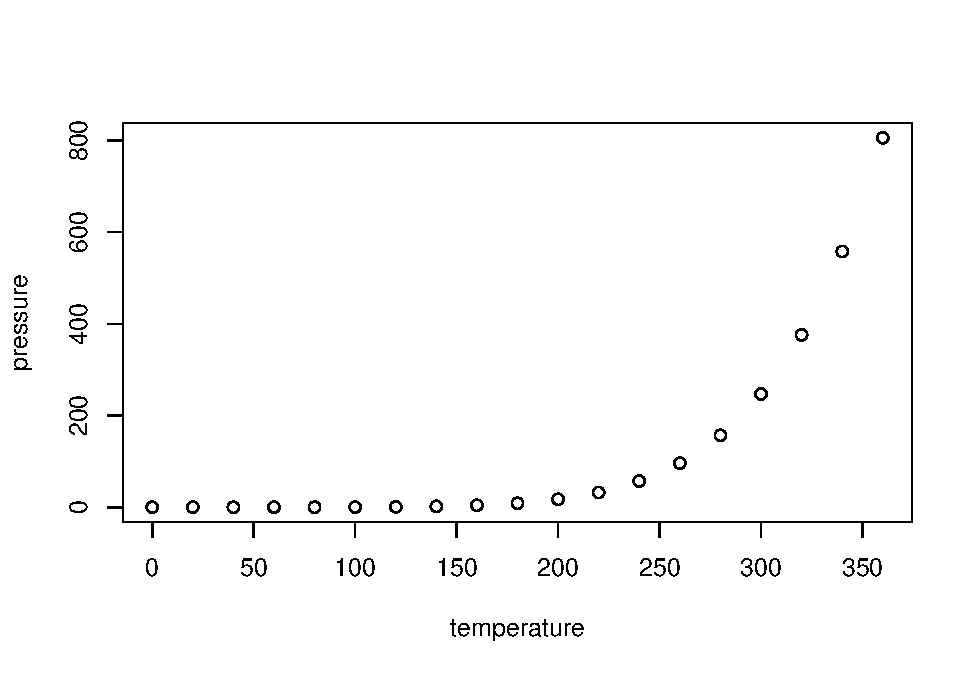
\includegraphics{aquasat_outline_files/figure-latex/unnamed-chunk-3-1.pdf}

\hypertarget{map}{%
\subsection{Map}\label{map}}

\includegraphics{aquasat_outline_files/figure-latex/unnamed-chunk-4-1.pdf}

\hypertarget{spectral-library}{%
\subsection{Spectral library}\label{spectral-library}}

\hypertarget{spectral-medians-captured-at-sample-sites}{%
\subsubsection{Spectral medians captured at sample
sites}\label{spectral-medians-captured-at-sample-sites}}

\includegraphics{aquasat_outline_files/figure-latex/unnamed-chunk-5-1.pdf}

\hypertarget{spectral-variation-captured-by-our-circles}{%
\subsubsection{Spectral variation captured by our
circles}\label{spectral-variation-captured-by-our-circles}}

\begin{verbatim}
## Warning in self$trans$transform(x): NaNs produced
\end{verbatim}

\begin{verbatim}
## Warning: Transformation introduced infinite values in continuous x-axis
\end{verbatim}

\begin{verbatim}
## Warning: Removed 9988 rows containing non-finite values (stat_density).
\end{verbatim}

\includegraphics{aquasat_outline_files/figure-latex/unnamed-chunk-6-1.pdf}

\hypertarget{in-situ-library}{%
\subsection{In situ library}\label{in-situ-library}}

\hypertarget{all-parameters-no-type-breakdown}{%
\subsubsection{All parameters no type
breakdown}\label{all-parameters-no-type-breakdown}}

\begin{verbatim}
## Warning: Removed 7228 rows containing non-finite values (stat_boxplot).
\end{verbatim}

\includegraphics{aquasat_outline_files/figure-latex/unnamed-chunk-7-1.pdf}

\hypertarget{dominant-groupings}{%
\subsection{Dominant groupings}\label{dominant-groupings}}

\includegraphics{aquasat_outline_files/figure-latex/unnamed-chunk-8-1.pdf}

\begin{verbatim}
##   r.squared adj.r.squared     sigma statistic p.value df    logLik
## 1 0.4316539     0.4315847 0.4337034   6238.84       0  5 -19174.51
##        AIC      BIC deviance df.residual
## 1 38361.02 38411.42 6180.544       32858
\end{verbatim}


\end{document}
